\documentclass{article}
\usepackage{subfiles}
\usepackage{graphicx} % Required for inserting images
\usepackage{ctex}
\usepackage{geometry}
\geometry{a4paper,scale=0.9}

\usepackage{amsmath} 
\usepackage{amssymb}
\usepackage{amsthm}
\usepackage{mathrsfs}
\usepackage{graphicx}
\usepackage{tikz}
\usepackage{bm}
\usepackage{bbm}

\begin{document}
\title{多车道场景MARL策略设计}
\author{}
\date{}
\maketitle
\section{基础框架}

\begin{center}
\begin{tikzpicture}[node distance=4.5cm,auto,>=latex]
    \node (env) {环境交互与特征处理};
    \node (sur_intention) [right of=env] {周围车辆意图预测};
    \node (sur_occupancy) [right of=sur_intention] {周围车辆占用预测};

    \node (lateral_decison) [below of=env] {横向决策与控制};
    \node (MARL) [right of=lateral_decison] {基于预测MARL的纵向控制};
    \node (safety) [right of=MARL] {安全评估机制};

    \node (evaluation) [below of=lateral_decison] {交通指标评估};
    \node (memory) [right of=evaluation] {执行轨迹存储};
    \node (CQR_update) [right of=memory] {CQR更新};

    \draw[->] (env) -- (sur_intention);
    \draw[->] (sur_intention) -- (sur_occupancy);
    \draw[->] (env) to[bend left] (sur_occupancy);

    \draw[->] (env) -- (lateral_decison);
    \draw[->] (lateral_decison) -- (MARL);
    \draw[->] (sur_occupancy) -- (safety);
    \draw[->] (safety) -- (MARL);

    \draw[->] (evaluation) -- (lateral_decison);
    \draw[->] (evaluation) -- (MARL);
    \draw[->] (MARL) -- (memory);
    \draw[->] (memory) -- (CQR_update);
    \draw[->] (lateral_decison) -- (sur_intention);

    \draw[->] (env) to[bend right] (evaluation);
    \draw[->] (CQR_update) to[bend right] (sur_occupancy);
\end{tikzpicture}
\end{center}

车辆相对关系示意图:

\begin{center}
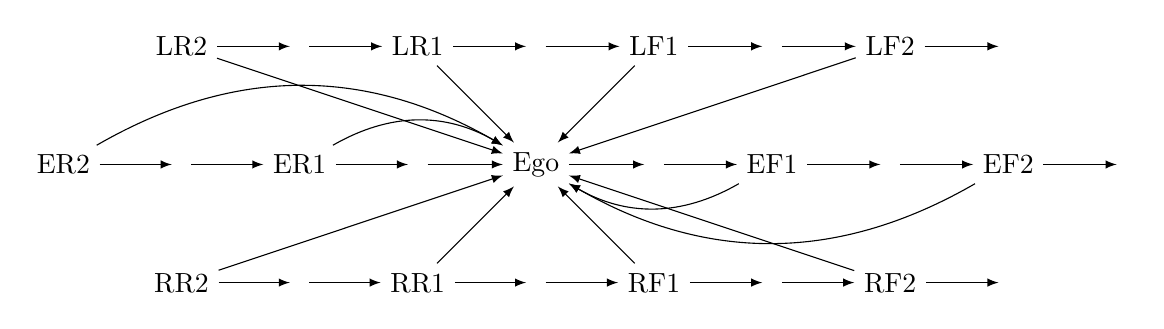
\begin{tikzpicture}[node distance=1.5cm,auto,>=latex]
    \node (none11) {};
    \node (LR2) [right of=none11] {LR2};
    \node (none12) [right of=LR2] {};
    \node (LR1) [right of=none12] {LR1};
    \node (none13) [right of=LR1] {};
    \node (LF1) [right of=none13] {LF1};
    \node (none14) [right of=LF1] {};
    \node (LF2) [right of=none14] {LF2};
    \node (none15) [right of=LF2] {};

    \node (ER2) [below of=none11] {ER2};
    \node (none21) [right of=ER2] {};
    \node (ER1) [right of=none21] {ER1};
    \node (none22) [right of=ER1] {};
    \node (Ego) [right of=none22] {Ego};
    \node (none23) [right of=Ego] {};
    \node (EF1) [right of=none23] {EF1};
    \node (none24) [right of=EF1] {};
    \node (EF2) [right of=none24] {EF2};
    \node (none25) [right of=EF2] {};

    \node (none31) [below of=ER2] {};
    \node (RR2) [right of=none31] {RR2};
    \node (none32) [right of=RR2] {};
    \node (RR1) [right of=none32] {RR1};
    \node (none33) [right of=RR1] {};
    \node (RF1) [right of=none33] {RF1};
    \node (none34) [right of=RF1] {};
    \node (RF2) [right of=none34] {RF2};
    \node (none35) [right of=RF2] {};

    % \draw[->] (none11) -- (LR2);
    \draw[->] (LR2) -- (none12);
    \draw[->] (none12) -- (LR1);
    \draw[->] (LR1) -- (none13);
    \draw[->] (none13) -- (LF1);
    \draw[->] (LF1) -- (none14);
    \draw[->] (none14) -- (LF2);
    \draw[->] (LF2) -- (none15);

    % \draw[->] (none11) -- (ER2);
    \draw[->] (ER2) -- (none21);
    \draw[->] (none21) -- (ER1);
    \draw[->] (ER1) -- (none22);
    \draw[->] (none22) -- (Ego);
    \draw[->] (Ego) -- (none23);
    \draw[->] (none23) -- (EF1);
    \draw[->] (EF1) -- (none24);
    \draw[->] (none24) -- (EF2);
    \draw[->] (EF2) -- (none25);


    % \draw[->] (none31) -- (RR2);
    \draw[->] (RR2) -- (none32);
    \draw[->] (none32) -- (RR1);
    \draw[->] (RR1) -- (none33);
    \draw[->] (none33) -- (RF1);
    \draw[->] (RF1) -- (none34);
    \draw[->] (none34) -- (RF2);
    \draw[->] (RF2) -- (none35);

    \draw[->] (LR2) -- (Ego);
    \draw[->] (LR1) -- (Ego);
    \draw[->] (LF1) -- (Ego);
    \draw[->] (LF2) -- (Ego);
    \draw[->] (ER2) to[bend left] (Ego);
    \draw[->] (ER1) to[bend left] (Ego);
    \draw[->] (EF1) to[bend left] (Ego);
    \draw[->] (EF2) to[bend left] (Ego);
    \draw[->] (RR2) -- (Ego);
    \draw[->] (RR1) -- (Ego);
    \draw[->] (RF1) -- (Ego);
    \draw[->] (RF2) -- (Ego);
\end{tikzpicture}
\end{center}
\section{特征处理模块}
请认真读取以下每个模块的特征需求,并在环境交互模块中完成对应特征的提取与处理,
确保每个模块均能正确获取所需特征输入。
总体来说我们需要提取的特征包含:
\begin{itemize}
    \item 交通环境状态:各车道的平均速度、车道密度;
    \item 所有车辆当前时刻状态:当前时刻的纵向位置$x$、横向位置$y$、速度$v$、加速度$a$、航向角$\theta$、车辆类型编码表示;
    \item 所有车辆历史时刻状态:历史20个时刻的纵向位置$x$、横向位置$y$、速度$v$、加速度$a$、航向角$\theta$、车辆类型编码表示;
    \item 以每辆车为中心(Ego)的周围车辆特征:车辆名称、当前时刻的纵向位置$x$、横向位置$y$、速度$v$、加速度$a$、航向角$\theta$,以及与Ego车辆的相对位置$\Delta x_{*}$、相对横向位置$\Delta y_{*}$、相对速度$\Delta v_{*}$、纵向碰撞时间$T_{*}$
\end{itemize}

% 把所有的特征提取函数都放在01_MARL_MultiLane/MARL_MultiLane/harl/envs/a_multi_lane/env_utils/feature_extractor.py文件中。

\section{CAV横向决策与控制}
横向决策分为向左变道概率计算、向右变道概率计算、保持车道概率计算三部分,
根据三者概率大小决定最终横向动作。
向左变道概率计算、向右变道概率计算与基于SCM的横向意图预测(概率输出)的逻辑一致,我们依次以左车道、右车道作为目标车道进行特征提取与概率计算。
\subsection{特征输入}
\textbf{交通特征:}
\begin{itemize}
    \item 各车道的统计信息:平均速度、车道密度;
    \item 本车道与目标车道的平均速度差、密度差;
    \item 以上四个特征组成交通环境状态矩阵,并进行归一化得到环境层因果机制的输入:
    $\mathbf{S}(t) = [\bar{v}_{EL}(t), \kappa_{EL}(t), \Delta \bar{v}(t), \Delta \kappa(t)]^T$
\end{itemize}
以上特征组成交通环境状态。

\textbf{Ego车辆特征:}
\begin{itemize}
    \item 当前时刻的纵向位置$x^i$、横向位置$y^i$、速度$v^i$、加速度$a^i$、航向角$\theta^i$;
    \item 车辆类型one-hot编码表示;
\end{itemize}
\textbf{周围车辆特征:}
\begin{itemize}
    \item 当前时刻的纵向位置$x_{*}^i$、横向位置$y_{*}^i$、速度$v_{*}^i$、加速度$a_{*}^i$、航向角$\theta_{*}^i$,其中*代表方位(EF1/TF1/TR1等),车辆方位标记如车辆相对关系示意图所示;
    \item 处理为相对特征:与Ego车辆的相对位置$\Delta x_{*}^i$、相对横向位置$\Delta y_{*}^i$、距离$d_{*}^i$、相对速度$\Delta v_{*}^i$、纵向碰撞时间$T_{*}^i$;
    \item 将以上特征整理为个体层因果机制的输入特征向量(需进行归一化):
    \begin{itemize}
        \item 必要性路径: $\varphi_N = [v^i, \Delta v_{\text{EF1}}^i, d_{\text{EF1}}^i, T_{\text{EF1}}^i]^T \in \mathbb{R}^4$,对应$\varphi_N = [v_{\text{ego}}, v_{\text{rel}}, d_{\text{headway}}, T_{\text{headway}}]^T \in \mathbb{R}^4$;
        \item 可行性路径: $\varphi_F = [v^i, \Delta v_{\text{TF1}}^i, d_{\text{TF1}}^i, T_{\text{TF1}}^i]^T \in \mathbb{R}^4$,对应$\varphi_F = [v_{\text{ego}}, \Delta v_{\text{adj,front}}, d_{\text{adj,front}}, T_{\text{adj,front}}]^T \in \mathbb{R}^4$;
        \item 安全性路径: $\varphi_S = [v^i, \Delta v_{\text{TR1}}^i, d_{\text{TR1}}^i, T_{\text{TR1}}^i]^T \in \mathbb{R}^4$,对应$\varphi_S = [v_{\text{ego}}, \Delta v_{\text{adj,rear}}, d_{\text{adj,rear}}, T_{\text{adj,rear}}]^T \in \mathbb{R}^4$;
    \end{itemize}
\end{itemize}

% 这里的相对信息计算以及特征归一化请参考00_Intention_Prediction/LCIntention/00_intention_prediction/feature_extraction.py文件中的相关定义。

\subsection{模型调用与横向决策输出}
调用已训练好的意图预测模型参数作为横向决策模型的基础参数,
并将上述特征输入模型进行向左变道概率$P_{left}$、向右变道概率$P_{right}$输出。
保持车道的概率计算为:
\begin{equation}
    P_{keep} = 1 - \max(P_{left}, P_{right})
\end{equation}
最终横向决策输出为:
\begin{equation}
    D_{lat} = \arg\max_{d \in \{left, keep, right\}} P_d
\end{equation}

\subsection{横向控制输出}
根据以上横向决策模型输出的横向决策$D_{lat}$,结合当前车辆状态,
调用横向控制模块生成具体的横向控制指令(如横向加速度$a_{lat}$),并输出至环境交互模块。
横向轨迹设计为贝塞尔曲线形式:
\begin{equation}
y_{\text{ref}}(t) = \sum_{i=0}^{4} B_i^4(u) P_i
\end{equation}
参数化变量 $u = \frac{t}{t_{LC}} \in [0,1]$,四阶伯恩斯坦基函数:
\begin{equation}
B_i^4(u) = \binom{4}{i}(1-u)^{4-i}u^i
\end{equation}

控制点设置:
\begin{equation}
P_0 = y_0, \quad P_1 = y_0 , \quad P_2 = \frac{y_0 + y_{\text{target}}}{2}
\end{equation}
\begin{equation}
P_3 = y_{\text{target}}, \quad P_4 = y_{\text{target}}
\end{equation}

其中,$\Delta y = y_{\text{target}} - y_0$。

\textbf{速度轨迹:}
\begin{equation}
v_{\text{ref},x}(t) = a_1 + 2a_2t + 3a_3t^2
\end{equation}
\begin{equation}
v_{\text{ref},y}(t) = \frac{4}{t_{LC}} \sum_{i=0}^3 B^3_i\left(\frac{t}{t_{LC}}\right) (P_{i+1} - P_i)
\end{equation}

\textbf{加速度轨迹:}
\begin{equation}
a_{ref,x}(t) = 2a_2 + 6a_3t
\end{equation}
\begin{equation}
a_{ref,y}(t) = \frac{12}{t^2_{LC}} \sum_{i=0}^2 B^2_i\left(\frac{t}{t_{LC}}\right) (P_{i+2} - 2P_{i+1} + P_i)
\end{equation}

\subsection{决策模型更新}
首先需要设置一个经验回放池,保存CAV横向决策模型的执行轨迹数据,供后续模型更新使用。
横向决策模型使用CAV执行轨迹进行SCM模型更新。
可调参数为环境层的因果机制参数以及环境-个体因果门控融合机制参数,个体层的因果机制参数保持不变。
CAV的横向决策目标为促进交通效率,同时要惩罚不安全的横向决策,因此横向决策模型更新的损失函数设计为:
\begin{equation}
    \mathcal{L}(\theta_E) = \sum_{t=1}^{T} \left( - \omega_{efficiency} \mathcal{L}_{efficiency}(t) + \omega_{safe} \mathcal{L}_{safe}(t) \right)
\end{equation}
其中,$\mathcal{L}_{efficiency}(t)$为交通效率损失,$\mathcal{L}_{safe}(t)$为安全损失,$\omega_{efficiency}$与$\omega_{safe}$分别为对应的权重系数。
交通效率损失定义为整体车辆的平均速度损失,当整体车辆速度提升时损失减小:
\begin{equation}
    \mathcal{L}_{efficiency}(t) = 1 - \frac{1}{N} \sum_{i=1}^{N} v^i(t)
\end{equation}

在计算安全损失时首先识别出训练批次中不安全的横向决策行为,也就是变道过程中与周围车辆发生碰撞的情况,
建立不安全样本集合:
\begin{equation}
\mathcal{I}_{\text{unsafe}} = \left\{i \in \{1, \ldots, B\} : P_{\text{safety}}^{(i)} < \theta\right\}
\label{eq:unsafe_set}
\end{equation}

其中:
\begin{itemize}
    \item $P_{\text{safety}}^{(i)} = \sigma(S^{(i)} = \frac{1}{1 + e^{-S^{(i)}}} \in (0, 1))$: 第 $i$ 个样本的安全性路径概率输出通过sigmoid函数转换为概率:
    \item $\theta \in [0.3, 0.4]$: 安全阈值,默认0.3
\end{itemize}

\textbf{安全阈值的语义}: 
\begin{itemize}
    \item $P_{\text{safety}} < \theta$: 安全性路径判定为``不安全''
    \item $P_{\text{safety}} \geq \theta$: 安全性路径判定为``安全''或``中性''
\end{itemize}

\paragraph{违约样本的惩罚}

对于不安全样本,若最终预测概率超过允许的最大值 $\epsilon_{\max}$,则视为违约并施加二次惩罚:

\begin{equation}
\mathcal{L}_{\text{safety}} = \begin{cases}
\displaystyle\frac{1}{|\mathcal{I}_{\text{unsafe}}|} \sum_{i \in \mathcal{I}_{\text{unsafe}}} \left[\max\left(0, P_{\text{final}}^{(i)} - \epsilon_{\max}\right)\right]^2 & \text{if } |\mathcal{I}_{\text{unsafe}}| > 0 \\
0 & \text{otherwise}
\end{cases}
\label{eq:safety_loss}
\end{equation}

其中 $\epsilon_{\max} \in [0.05, 0.15]$ 是最大允许违约概率,默认0.1。

% 将横向决策模型调用、输出与更新的代码放在01_MARL_MultiLane/MARL_MultiLane/harl/envs/a_multi_lane/env_utils/lateral_decision.py文件中。
同时需要注意保存决策模型更新所需的执行轨迹数据至经验回放池,供后续模型更新使用。
模型更新后需及时同步更新横向决策模型参数。

\section{周围车辆意图预测}
\subsection{特征输入}
与横向决策模型类似,调用已训练好的SCM意图预测模型结构与参数,以被预测的车辆(目标车辆)为中心,作为Ego车辆,目标车辆周围的车辆作为环境车辆,
并将以下特征输入模型进行意图预测。
\begin{itemize}
    \item 交通环境特征:各车道的平均速度、车道密度,本车道与目标车道的平均速度差、密度差,组成环境层因果机制的输入;
    \item Ego车辆特征:当前时刻的纵向位置$x$、横向位置$y$、速度$v$、加速度$a$、航向角$\theta$、车辆类型编码表示;
    \item 周围车辆特征:当前时刻的纵向位置$x$、横向位置$y$、速度$v$、加速度$a$、航向角$\theta$,以及与Ego车辆的相对位置$\Delta x_{*}$、相对横向位置$\Delta y_{*}$、相对速度$\Delta v_{*}$、纵向碰撞时间$T_{*}$,组成个体层因果机制的输入特征向量。
\end{itemize}

特征提取与归一化同横向决策模型。
\subsection{模型调用}
分为HDV意图预测与CAV意图预测两部分,HDV意图预测模型直接调用已训练好的SCM意图预测模型参数进行意图预测输出,
CAV意图预测模型则调用已训练好的HDV意图预测模型参数作为CAV意图预测模型的基础参数,
并将上述特征输入模型进行意图预测输出。

与横向预测相同,意图预测输出为向左变道概率$P_{left}$、向右变道概率$P_{right}$,保持车道概率$P_{keep}$计算为:
\begin{equation}
    P_{keep} = 1 - \max(P_{left}, P_{right})
\end{equation}
最终意图预测输出为:
\begin{equation}
    I_{lat} = \arg\max_{d \in \{left, keep, right\}} P_d
\end{equation}

\subsection{CAV意图预测模型更新}
与CAV横向决策模型更新同步进行,从CAV横向决策模型保存文件夹中读取最新的模型参数,不需要计算损失函数与反向传播更新。

\section{周围车辆未来占用预测}
\subsection{特征输入}
同样以被预测的车辆(目标车辆)作为Ego车,目标车辆周围车辆作为周车,基于CQR的占用预测模型输入:
\begin{itemize}
    \item 交通环境特征:各车道的平均速度、车道密度;
    \item Ego车辆的历史轨迹信息:每个时刻均包含相对当前时刻的位置(横纵向)、相对当前时刻的速度、实时加速度、实时航向角、车辆类型;
    \item 周车的历史轨迹信息:每个时刻均包含相对Ego当前时刻的位置(横纵向)、相对Ego当前时刻的速度、实时加速度、实时航向角、车辆类型;
    \item 意图预测模块输出的Ego车横向意图。
\end{itemize}

% 特征提取与归一化过程请参考00_Occupancy_Prediction/OccupancyPred/00_trajectory_prediction/feature_extraction.py中的相关定义。
% 另外特征使用请参考00_Occupancy_Prediction/OccupancyPred/00_trajectory_prediction/CQR_SCM_design/data_loader.py文件中的相关定义。
\subsection{模型调用}
对于HDV占用预测与CAV占用预测,均调用已训练好的CQR模型参数进行占用预测输出。
但均存储被预测HDV和CAV的执行轨迹至经验回放池,供后续CQR模型更新使用。

\subsection{CQR模型更新}
HDV占用预测模型使用HDV执行轨迹进行CQR模型更新,CAV占用预测模型使用CAV执行轨迹进行CQR模型更新。
每隔固定时间间隔(如每100个训练回合)进行一次CQR模型更新。
更新时仅进行共形化校准更新,不进行QR模型参数更新。
CAV共形化校准参数与HDV共形化校准参数分开存储与更新。

\section{安全惩罚机制}
在环境中读取Ego车辆更新的位置$x^i_{ego}(t+1)$以及上一时刻的位置$x^i_{ego}(t)$,因此产生了由动作$a^i_{ego}(t)$引起的位置变化范围$O^i_{ego}(t) = [x^i_{ego}(t), x^i_{ego}(t+1)]$。
基于周围车辆未来占用预测结果,评估Ego车辆位置变化范围$O^i_{ego}(t)$与周围车辆未来占用范围$O^i_{i}(t)$的重叠情况。
\begin{equation}
    A_{overlap}(t) = O^i_{ego}(t) \cap \left( \bigcup_{j} O^i_{j}(t) \right), j \in \text{周车集合}
\end{equation}
进而,根据重叠面积$A_{overlap}(t)$计算安全惩罚值$R_{safe}(t)$:
\begin{equation}
    R_{safe}(t) = - \lambda \cdot \frac{A_{overlap}(t)}{A_{ego}(t)}
\end{equation}
其中,$A_{ego}(t)=x^i_{ego}(t+1) - x^i_{ego}(t)$为Ego车辆在时间$t$的位置变化范围面积,$\lambda$为惩罚系数。

% 定义一个单独的安全评估模块(safety_assessment.py),专门负责计算安全惩罚值$R_{safe}(t)$,并将其传递给MARL纵向控制模块作为奖励函数设计的一部分。

\section{基于预测性安全的MARL策略设计}
\subsection{状态空间}
\begin{itemize}
    \item 交通环境特征:各车道的平均速度、车道密度;
    \item Ego车辆的历史轨迹信息:每个时刻均包含相对当前时刻的位置(横纵向)、相对当前时刻的速度、实时加速度、实时航向角、车辆类型;
    \item 周车的历史轨迹信息:每个时刻均包含相对Ego当前时刻的位置(横纵向)、相对Ego当前时刻的速度、实时加速度、实时航向角、车辆类型;
\end{itemize}
\subsection{动作空间}
连续动作空间,纵向加速度$a_x \in [a_{min}, a_{max}]$;

\subsection{actor-critic网络设计}
actor网络使用含本车与周围车辆历史轨迹的状态空间:
\begin{itemize}
    \item 首先使用MLP对每个车的历史轨迹信息进行处理,然后使用图注意力网络对周围车辆的特征(历史轨迹特征+当前状态)进行融合得到周车交互特征表示。
    \item 对交通信息进行MLP处理得到交通特征表示。
    \item Ego车辆特征表示、周车交互特征表示与交通特征表示进行拼接后通过MLP处理,最终输出纵向加速度$a_x$。
\end{itemize}
% actor网络代码设计输出为01_MARL_MultiLane/MARL_MultiLane/harl/models/base/multi_lane/historical_encoder.py。

critic网络使用含有历史轨迹信息编码的状态空间:
\begin{itemize}
    \item 首先使用MLP对每个车的历史轨迹信息进行处理,然后使用图注意力网络对所有车辆的特征(历史轨迹特征+当前状态)进行融合得到车辆交互特征表示。
    \item 对交通信息进行MLP处理得到整体交通特征表示。
    \item 使用交叉注意力机制融合车辆交互特征表示与整体交通特征表示,最终通过MLP处理输出状态价值$V(s)$。
\end{itemize}
% critic网络代码设计输出为01_MARL_MultiLane/MARL_MultiLane/harl/models/value_function_models/historical_v_net.py。

\subsection{奖励函数设计}

\begin{equation}
    R(t) = \omega_{efficiency} R_{efficiency}(t) + \omega_{comfort} R_{comfort}(t) + \omega_{safe} R_{safe}(t)
\end{equation}
其中,$R_{efficiency}(t)$为交通效率奖励,$R_{comfort}(t)$为乘坐舒适度奖励,$R_{safe}(t)$为基于预测的安全惩罚奖励,$\omega_{efficiency}$、$\omega_{comfort}$与$\omega_{safe}$分别为对应的权重系数。

% 请参考现有代码实现奖励函数设计,代码路径为01_MARL_MultiLane/MARL_MultiLane/harl/envs/a_multi_lane/env_utils/veh_env_wrapper.py。

\section{SUMO环境交互}
% 这一章节的代码已在01_MARL_MultiLane/MARL_MultiLane/harl/envs/a_multi_lane/env_utils/veh_env_wrapper.py中定义。
\subsection{环境信息读取}
从环境读取每个时刻所有车辆的实时状态信息,包括位置、速度、加速度、航向角等。
\subsection{车辆控制输出}
发送给SUMO的横向控制仅为变道指令,纵向控制转换为速度指令。
\end{document}
